\chapter{粒子線に対する応答評価試験のための読み出しシステムの動作確認}
この章では,粒子線に対する応答評価試験のために行なった,外部トリガを処理する機能の追加と,応答評価試験のための準備について述べる.

\section{読み出しセットアップ概要}
以下に読み出しシステムの概要を示す.主にRD53A搭載のSingle Chip Card(SCC)とFPGAボード,PCを用いて読み出しシステムを構成している.今回は読み出しASICとFPGAボードは,HPC-mDP変換ボードを用いてケーブルにて接続を行い,FPGA内部でASICからのデータ信号の処理を行なった.また,高速通信用インターフェースでPCとFPGAボードを接続し,データ転送を行なった.\\

\subsection*{PC}
PCからPCIeによって接続されたFPGAボードに制御コマンドを送る.また,FPGAボードからきたデータを整理する.DAQの基本的なソフトウェアとファームウェアはYARRのDAQシステムを用いた.YARRは読み出しシステムの構築と性能向上を目指すオープンソースプロジェクトである.

\subsection*{FPGAボード}
Xilinx, Inc.のKintex-7 FPGA搭載KC705評価ボードを使用.このFPGAボードは,研究室規模の実験で使うことを想定しているため,FPGA評価ボードは一般的に流通してて入手性がよいため,このFPGAボードを使用している.また,KC705はPCIe通信に対応し,PCとPCIe間では5.12 $\mathrm{Gbps}$の通信速度に対応している.今回はYARRのシステムに外部トリガを受信,処理を行う機能を追加し,RD53Aの出力するHitOR信号を用いて,外部トリガを受信できているかを確認した.

\subsection*{アダプタカード}
ASICはDP-mDPケーブルからmDP-HPCアダプタカードを通してFPGAボードに接続される.

\subsection*{RD53A搭載Single Chip Cardモジュール}
ASICを1チップ搭載した試験用モジュールがSingle Chip Cardモジュールである.今回試験したのはアップグレード用のプロトタイプ版ASICであるRD53A搭載のモジュールである.
.センサ付きのRD53Aが搭載されたモジュールの写真を以下に示す.RD53Aは細い金属ワイヤにより基板上の回路パターンと電気的に接続されている.基板にRD53Aが外部と通信するためのDPコネクタ(図中:DP1),電源供給のためのmolexコネクタ(図中:PWR IN),センサに電圧を印加するためのLEMOコネクタ(図中:HV),センサが検出した信号を外部に出力するためのDPコネクタ(DP2)が実装されている.今回電源とセンサに印加した電圧は\ref{tab:voltage}に示す.

\begin{table}[h]
  \centering
  \caption{今回RD53Aとセンサに供給した電圧}
  \begin{tabular} {|l|cc|c|} \hline
     & RD53A & RD53A & ピクセル \\ 
     & アナログ回路 & デジタル回路 & センサ \\ \hline
    印加電圧[$\mathrm{V}$] & 1.80 & 1.80 & -50 \\ \hline
  \end{tabular}
  \label{tab:voltage}
\end{table}


\subsection*{$\beta$線源}
今回は粒子線として$\beta$線源であるストロンチウム90を使用した.使用した線源の現在の放射能は以下のように計算した.

\section{伝達確認}
ソーススキャンを行うために,既存のKC705用YARRファームウェアに外部トリガを処理する機能を追加した.本節では,機能を追加したファームが外部トリガを受信確認について述べる.

\subsection{コマンド信号とデータ信号の確認}
オシロスコープでコマンド信号とデータ信号をRD53A SCC上でプローブし,波形を確認した.

\subsection{デジタルスキャン}
全ピクセルのデジタル回路に複数回擬似パルスを注入して,注入した回数のうち何回応答が返ってくるのかを確認する.この作業をデジタルスキャンと呼ぶ.全ピクセルごとの回路の応答を確認し,データの転送線,FPGA内部の処理,PCへの通信の各経路でデータの損失がないことを確認するのに有効である.

\subsection{アナログスキャン}
アナログ回路に複数回擬似パルスを注入して,注入した回路のうち何回応答が返ってくるのかを確認した.この作業をアナログスキャンと呼ぶ.今回はDiff FEのみを使用するので,その他のフロントエンドは,グローバルレジスタの''CoreColEnSync1/2'',''CoreColEnLin1/2''を全て0にすることで非使用に設定した.また,Diff FE内接続されているピクセルセンサの上下構造の違いにより,上半分にノイズが多く現れるため,それを防ぐために,Diff FEのアナログ回路のLCC回路の部分をオンにする.これは,グローバルレジスタ''DiffLccEn''という値を0から1に変更し,''DiffLcc''を255にすることでオンにすることができる.以下にLCC回路をオフにした場合,オンにした場合それぞれのDiff FEのアナログスキャンの結果を示す.

\subsection{閾値のチューニング}
閾値とはピクセルの応答率が50$\mathrm{\%}$となる電荷量で定義される,ピクセルごと閾値を決めるDAC値を調節することによってピクセルごとの閾値を揃える.この作業を閾値のチューニングという.図\ref{fig:scurve}は,注入電荷を変化させながら,各ピクセルに試験電荷を複数回入射したときの応答数の概念図である.この閾値をチューニング目標値になるように,各ピクセルのパラメータを変更する.
\begin{figure}[h]
\centering
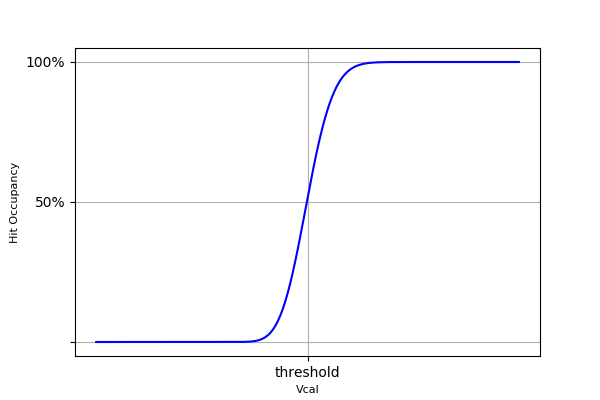
\includegraphics[width=8cm]{./figure/scurve.png}
\caption{注入電荷$V_{cal}$と応答率(HitOccupancy)の関係.応答率50$\mathrm{\%}$となる注入電荷が閾値となる}
\label{fig:scurve}
\end{figure}

閾値チューニング前後の各ピクセルの閾値のヒストグラムを示す.目標値は2500$\mathrm{e}$と設定した.\\
2500$\mathrm{e}$という閾値は,センサの厚みとノイズ信号の大きさを考慮した値である.今回使用したセンサの厚みは,150 $\mathrm{\mu m}$であり, 全て空乏化した場合に発生する信号は10000 $\mathrm{e}$である.まず,この信号をASICが読み出す際に,4分割されてしまったとしても,検出してほしいために閾値は2400 $\mathrm{e}$以下であることが望ましい.また,ノイズ$\sigma$の大きさに対して6-7 $\sigma$離れている必要があるため,バイアスレール有りの場合,$\sigma = 200 \mathrm{e}$と知られているため,1200 $\mathrm{e}$以上にすることが望ましい.閾値のヒストグラムを見ると,1200 $\mathrm{e}$にチューニングした場合は,1200 $\mathrm{e}$以下まで多く分布してしまっているため,今回は分布が1200 $\mathrm{e}$以上に収まるような,2500 $\mathrm{e}$を目標値としてチューニングを行なった.
%これは今回はDiff FEのみを使用したため,Diff FE内のピクセルのみをチューニング対象とした.入力する電荷の大きさを変化させながら,電荷を複数回それぞれのピクセルに注入し,注入回数のうち応答が帰ってくる割合から応答率を得る.信号が閾値を超えたかどうかでヒットと認識するかどうかの判定を行なっているが,信号いは正規分布に従うノイズが乗るため,信号がヒットとして認識される閾値に幅がある.そのため,注入電荷と応答率の関係は以下のようになり,この曲線をSカーブと呼ぶ.得られたSカーブを次式の誤差関数でフィッティングして,応答率が50 $\mathrm{\%}$になる閾値を求める.\\

%まず,アナログ回路にキャリブレーション用のテストパルス$V_{cal}$を複数回注入して,注入回数のうち,応答が返ってくる割合から応答率を得る.

\subsection{ノイズスキャン}
任意の周波数でトリガを発行し,その全トリガ数に対するのアナログ回路から何回応答が返ってくるのかを確認する.この作業をノイズスキャンと呼ぶ.ピクセルセンサが粒子線以外の信号に対して反応していないことを確認するために有効である.\\
この作業によって,粒子線以外の信号に対して反応している部分は非使用に設定される.引き続きDiff FEのみを使用した.任意の周波数でトリガを送り,その時のアナログ回路からの応答に対して,閾値を超えるものを非使用に設定する.この作業をノイズスキャンと呼ぶ.今回は20000 $\mathrm{Hz}$で5分間ノイズスキャンを行なった.以下にノイズスキャンを行う前と行なった後のOccupancy MapとEnable Pixel Mapを示す.

\subsection{HitOR信号の伝達確認}
モジュールの上に$\beta$線源を配置し,オシロスコープでHitOR信号をRD53A SCC上でプローブすることで,波形を確認した.また,FPGAまでHitOR信号が伝わっているかどうか,正常に処理され,そのタイミングでトリガが出力されているかどうかをVivadoのLogic Analyzerを用いて確認した.それが以下の図である.



このようにファームウェアに外部トリガを取得し,処理する機能を追加できていることを確認した.






